\section{Simulation Analysis}
\label{sec:simulation}

\subsection{Operating Point Analysis}

Table~\ref{tab:op} shows the simulated operating point results for the circuit
under analysis. Compared to the theoretical analysis results, one notices the
following differences: describe and explain the differences.

\begin{table}[h]
  \centering
  \begin{tabular}{|l|r|}
    \hline    
    {\bf Name} & {\bf Value [A or V]} \\ \hline
    @gb[i] & -2.00589e-01\\ \hline
@id[current] & 1.017967e+00\\ \hline
@r1[i] & 1.915709e-01\\ \hline
@r2[i] & -2.00589e-01\\ \hline
@r3[i] & -9.01783e-03\\ \hline
@r4[i] & 1.164729e+00\\ \hline
@r5[i] & -1.21856e+00\\ \hline
@r6[i] & 9.731579e-01\\ \hline
@r7[i] & 9.731579e-01\\ \hline
v(1) & 8.030092e+00\\ \hline
v(2) & 7.833907e+00\\ \hline
v(3) & 7.417135e+00\\ \hline
v(4) & 2.989101e+00\\ \hline
v(5) & 7.861734e+00\\ \hline
v(6) & 1.163284e+01\\ \hline
v(7) & 9.951293e-01\\ \hline
v(8) & 2.989101e+00\\ \hline

  \end{tabular}
  \caption{Operating point. A variable preceded by @ is of type {\em current}
    and expressed in Ampere; other variables are of type {\it voltage} and expressed in
    Volt.}
  \label{tab:op}
\end{table}

\lipsum[1-1]


\subsection{Transient Analysis}

Figure~\ref{fig:trans} shows the simulated transient analysis results for the
circuit under analysis. Compared to the theoretical analysis results, one
notices the following differences: describe and explain the differences.

\begin{figure}[h] \centering
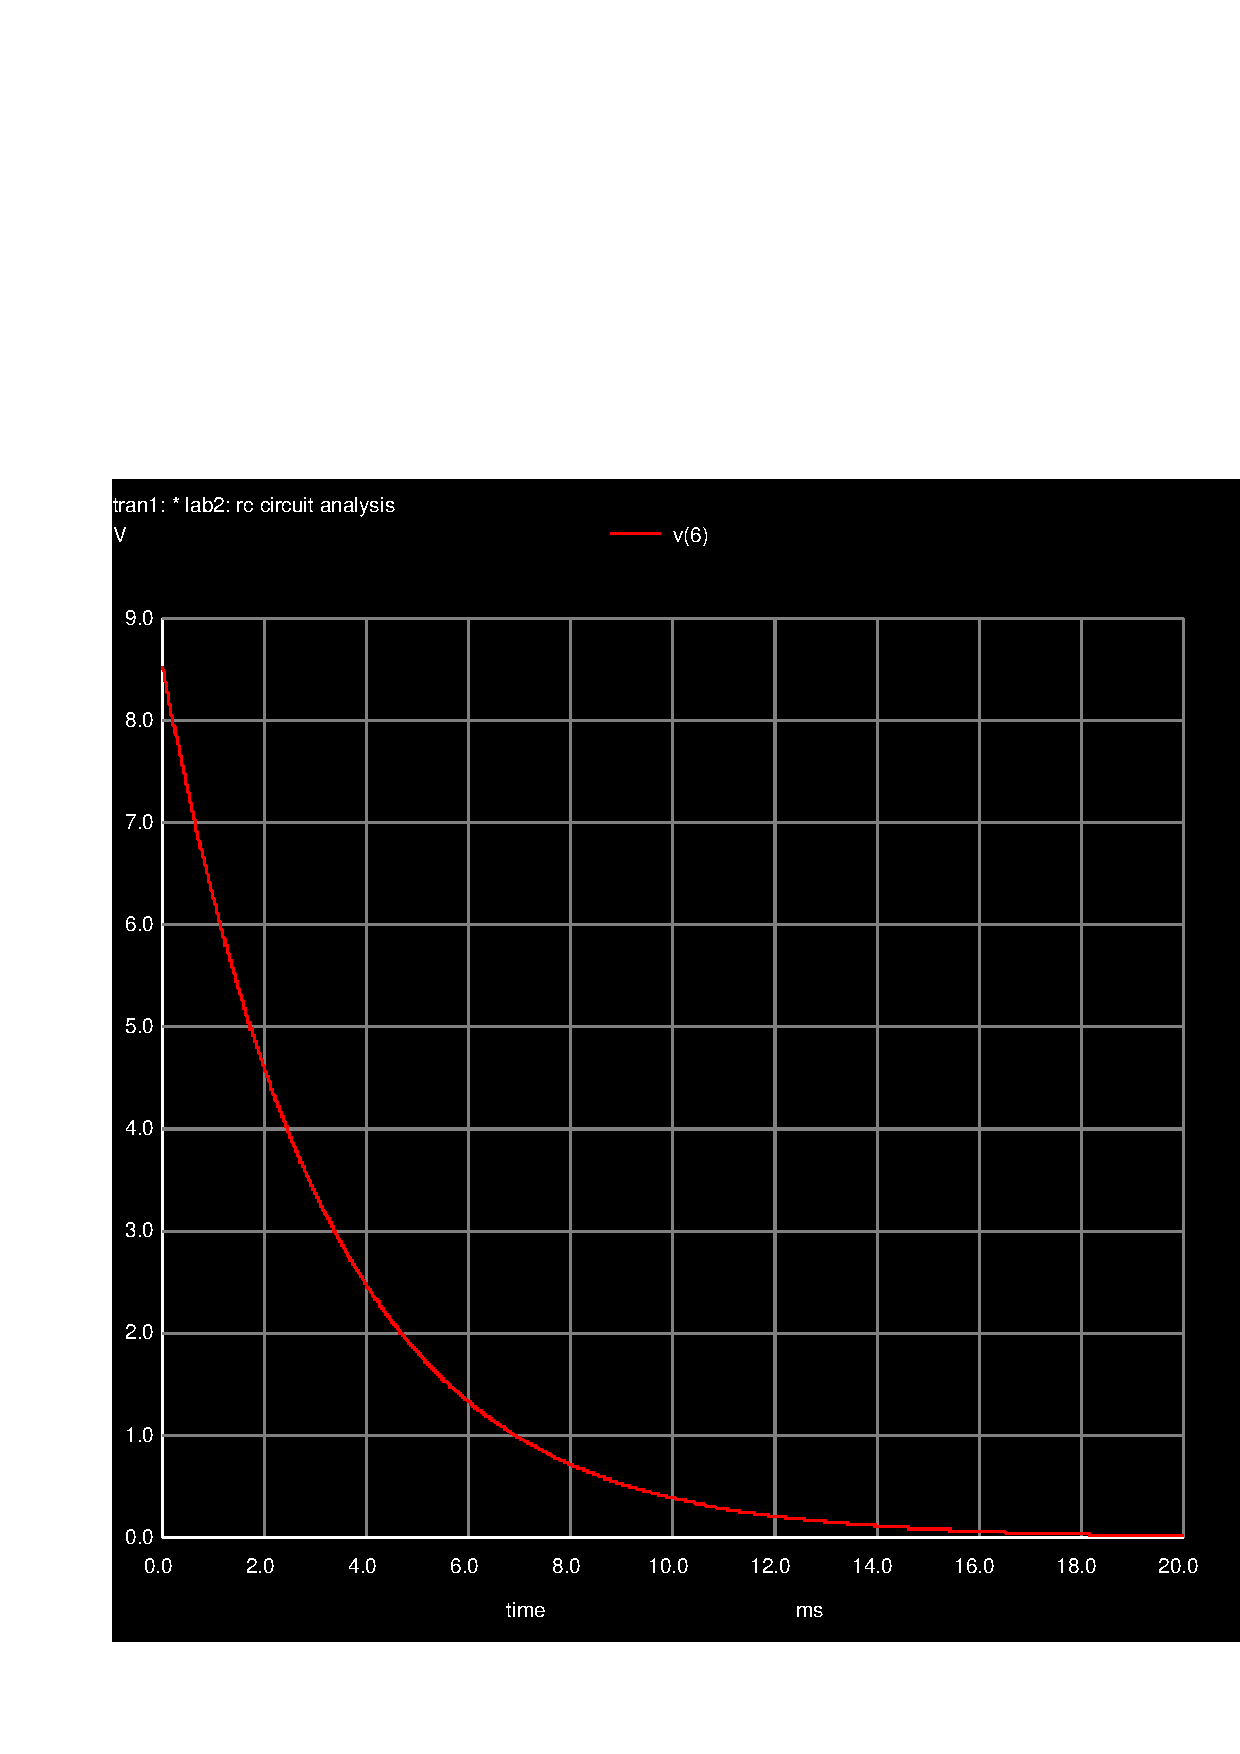
\includegraphics[width=0.6\linewidth]{trans.pdf}
\caption{Transient output voltage}
\label{fig:trans}
\end{figure}

\lipsum[1-1]



\subsection{Frequency Analysis}

\subsubsection{Magnitude Response}

Figure~\ref{fig:acm} shows the magnitude of the frequency response for the
circuit under analysis. Compared to the theoretical analysis results, one
notices the following differences: describe and explain the differences.

\begin{figure}[h] \centering
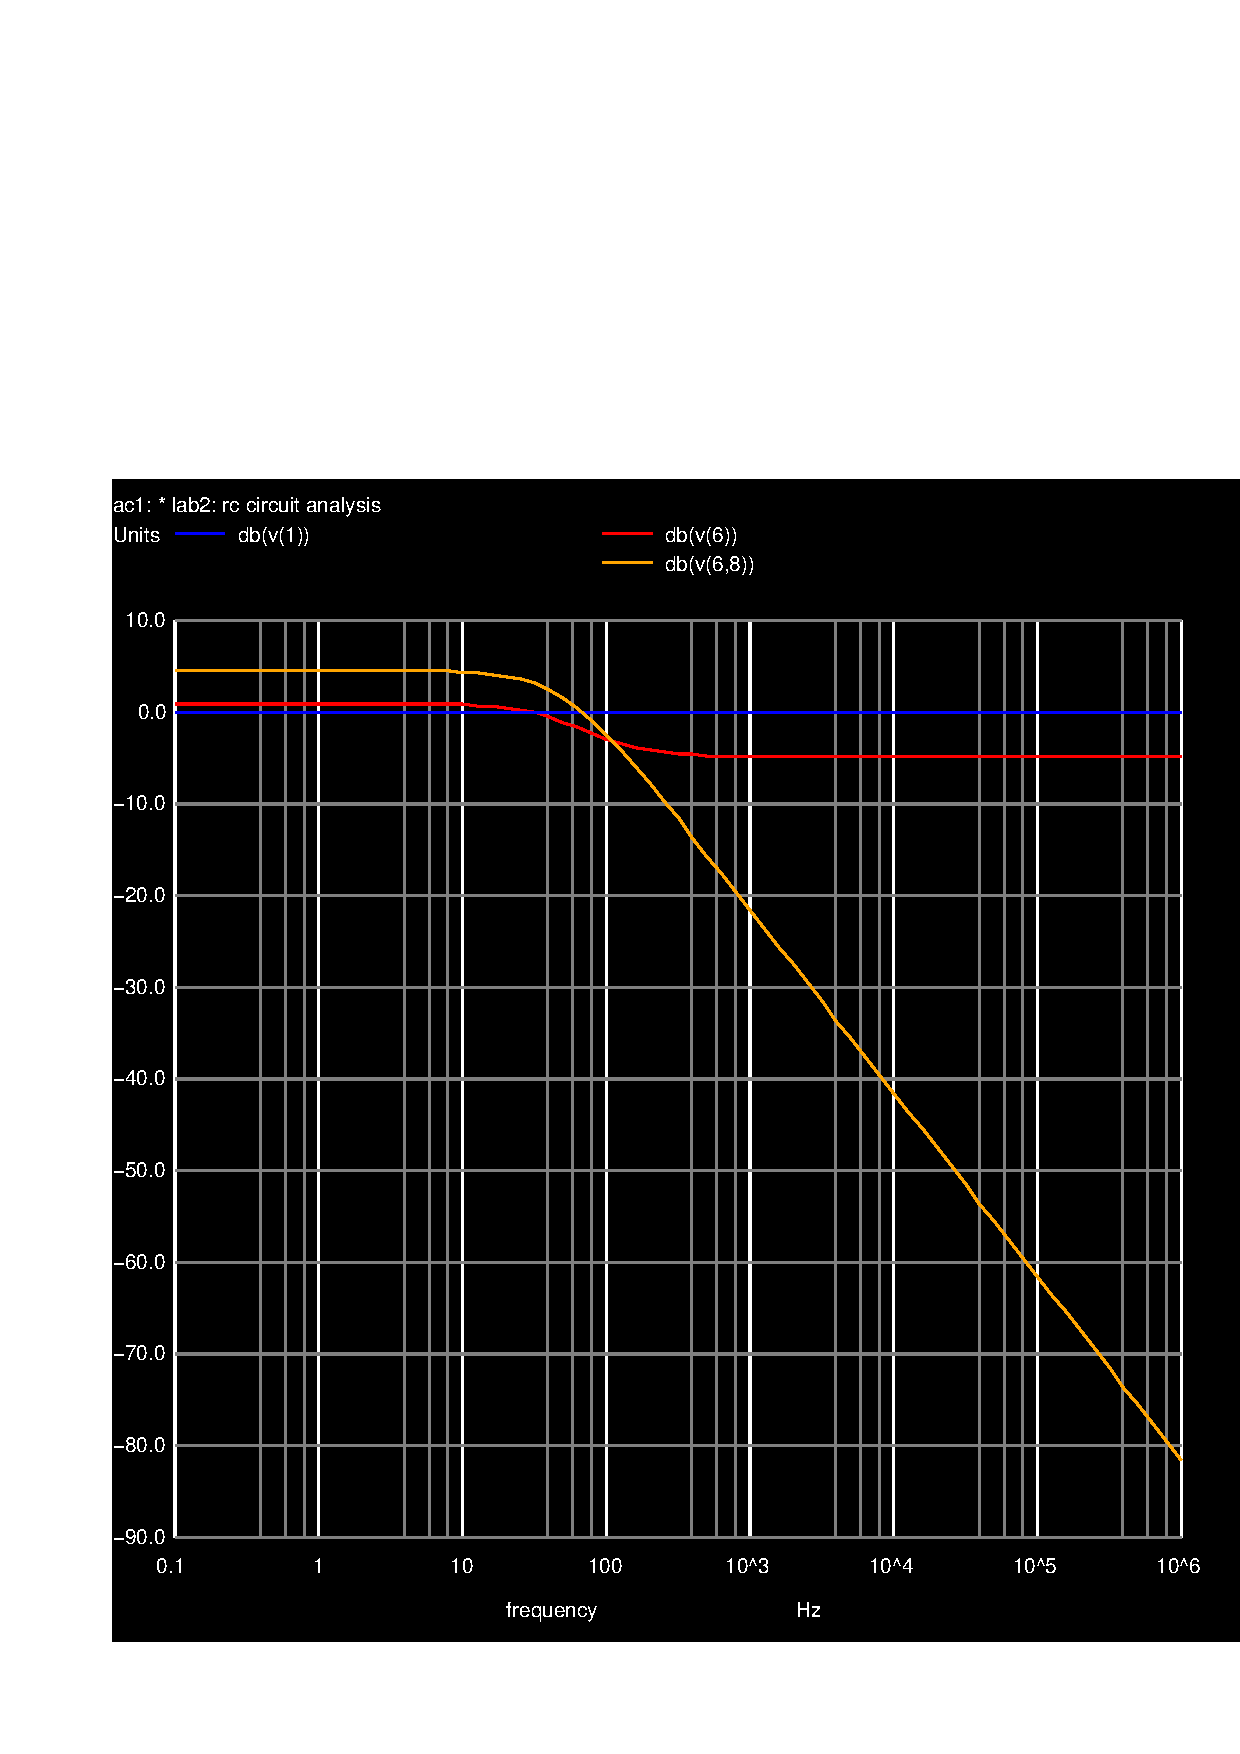
\includegraphics[width=0.6\linewidth]{acm.pdf}
\caption{Magnitude response}
\label{fig:acm}
\end{figure}

\lipsum[1-1]

\subsubsection{Phase Response}

Figure~\ref{fig:acp} shows the magnitude of the frequency response for the
circuit under analysis. Compared to the theoretical analysis results, one
notices the following differences: describe and explain the differences.

\begin{figure}[h] \centering
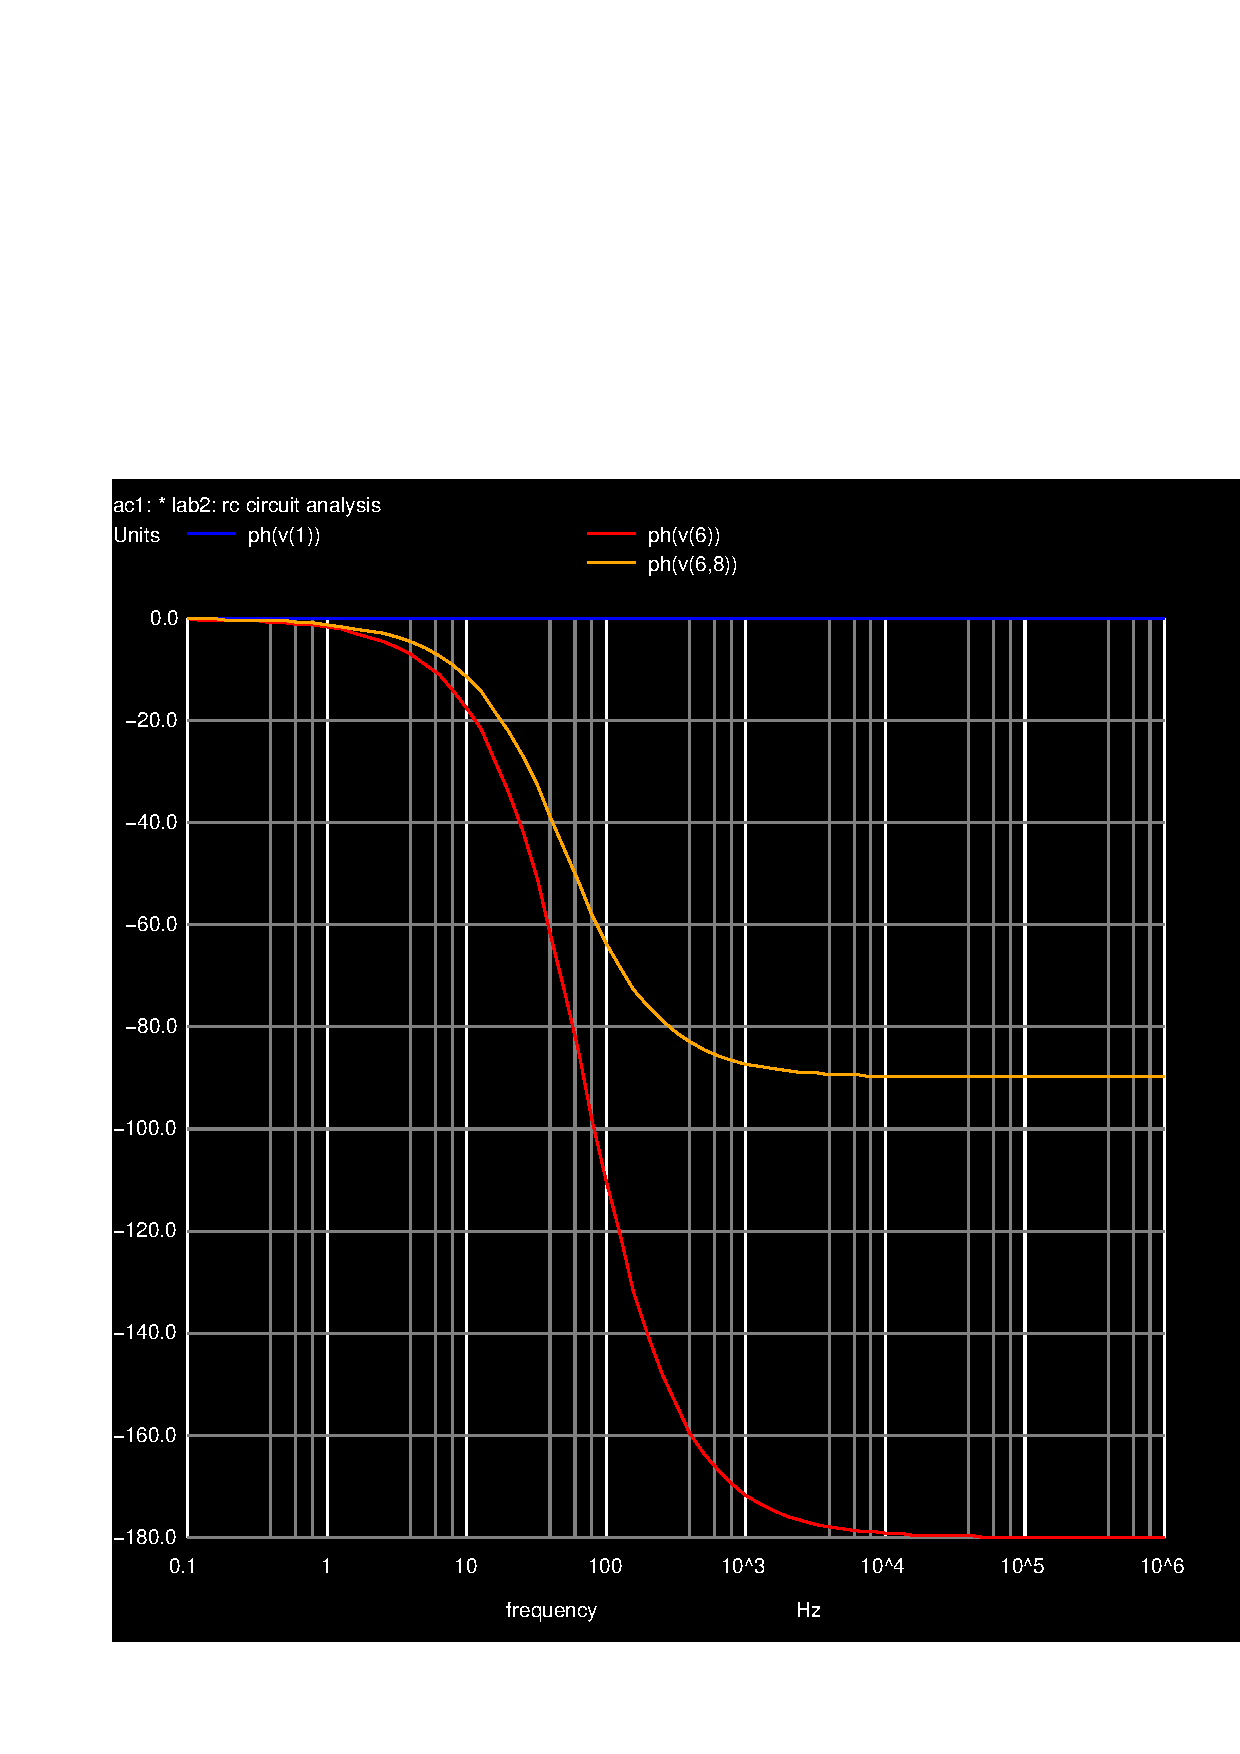
\includegraphics[width=0.6\linewidth]{acp.pdf}
\caption{Phase response}
\label{fig:acp}
\end{figure}

\lipsum[1-1]

\subsubsection{Input Impedance}

Figure~\ref{fig:zim} shows the magnitude of the frequency response for the
circuit under analysis. Compared to the theoretical analysis results, one
notices the following differences: describe and explain the differences.

\begin{figure}[h] \centering
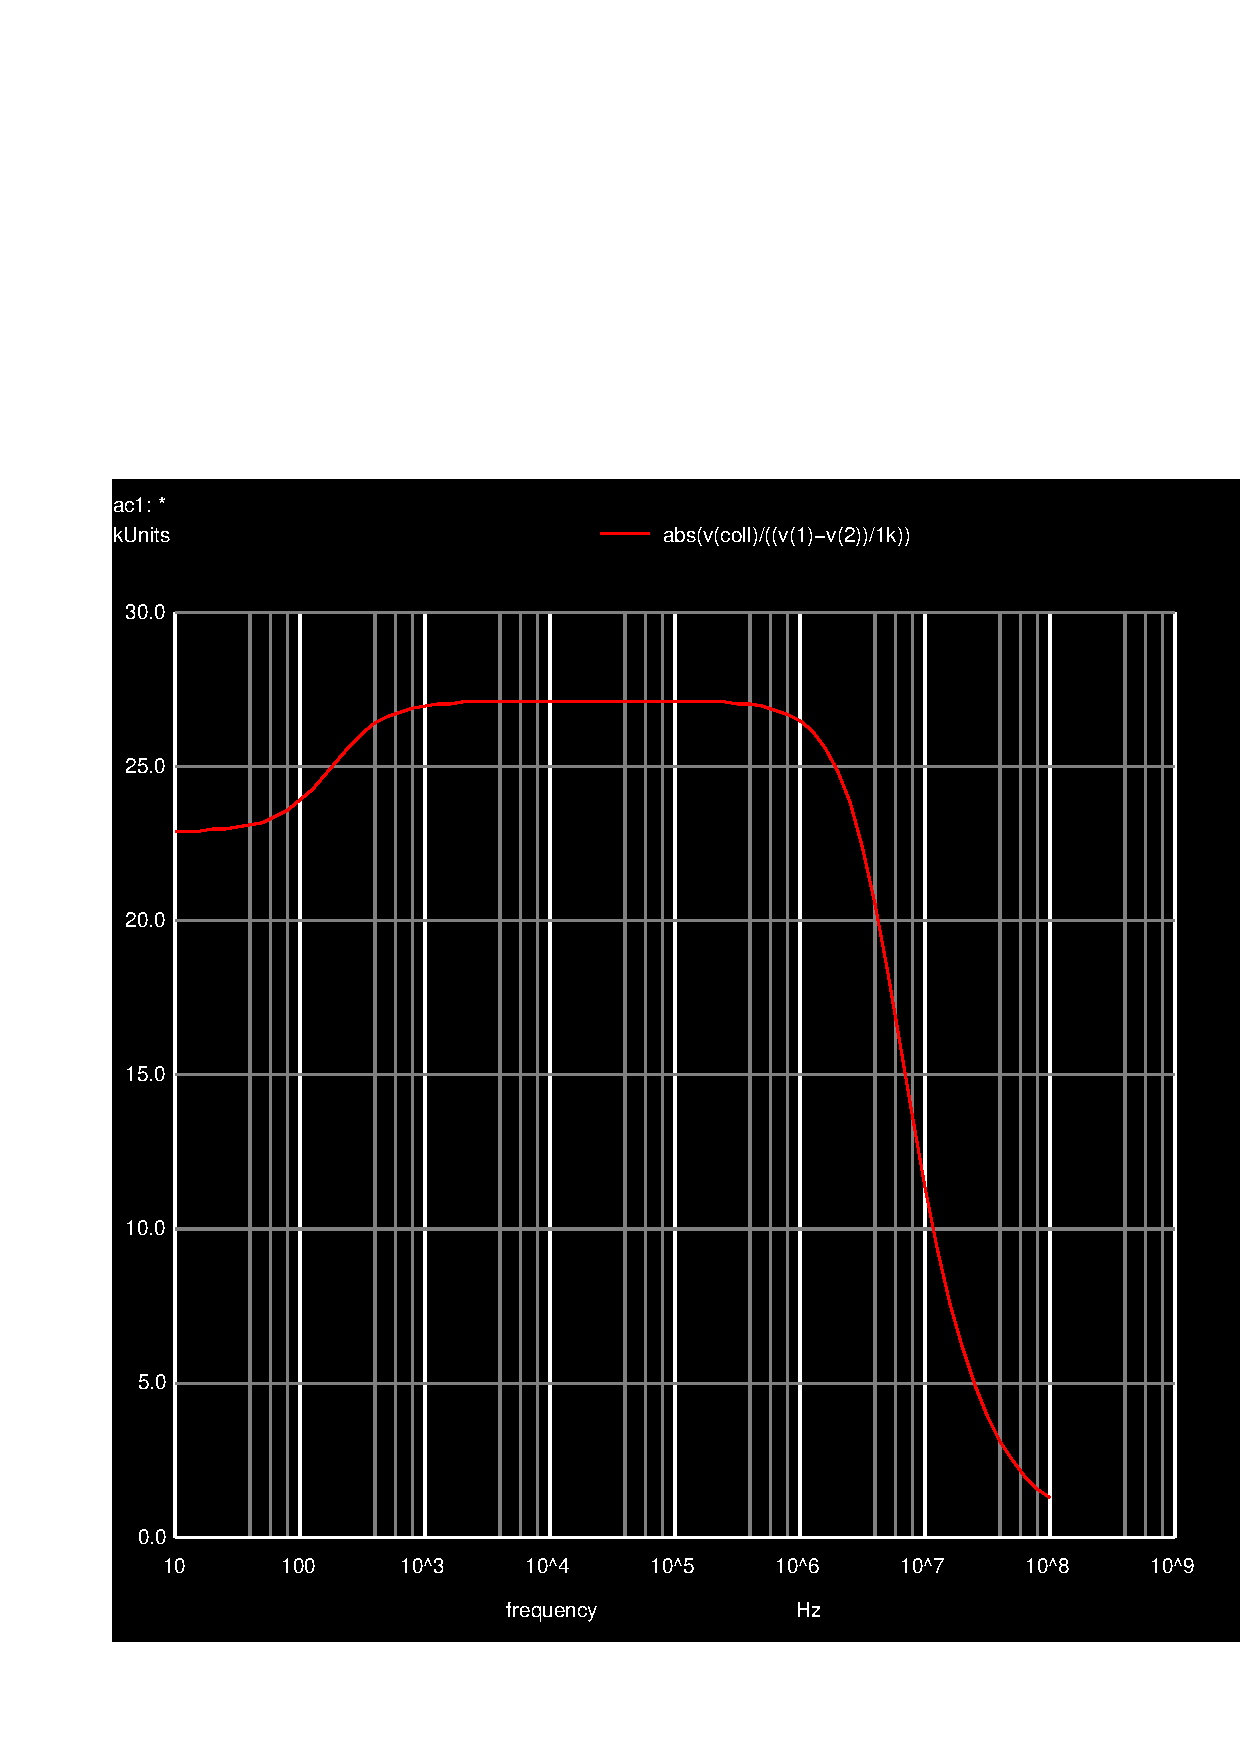
\includegraphics[width=0.6\linewidth]{zim.pdf}
\caption{Input impedance}
\label{fig:zim}
\end{figure}

\lipsum[1-1]



